\documentclass[11pt,compress]{beamer}
% deactivate beamer navigation
%\setbeamertemplate{navigation symbols}{}
%\usepackage{geometry}
%\geometry{papersize={180mm, 135mm}, top=-1.5mm} % 210mm, 297mm
\usepackage{../style/lmu-lecture}
\setbeamertemplate{frametitle}{\expandafter\uppercase\expandafter\insertframetitle}

\usepackage{tikz}

\usepackage{setspace}



\AtBeginSection[]
{
  \begin{frame}<beamer>
    \frametitle{Introduction to Machine Learning}
  \begin{minipage}{\textwidth}
  %decrease linespacing to display all points
  \linespread{0.01}\selectfont
  \begin{spacing}{0.001}
  \begin{small}
  \tableofcontents[currentsection, subsectionstyle=hide]
  \end{small}
  \end{spacing}
  \end{minipage}
  \end{frame}
}
% includepdf slides, pagecommad will set counter for framenumber
\usepackage{pdfpages}
\includepdfset{trim=0mm 0mm 0mm 0mm, pagecommand={\global\setcounter{framenumber}{\value{page}}}}
% trim=0mm 6mm 0mm 0mm, offset=0 15,
% add footer:
  \usepackage{framed, color}
\usepackage{xcolor}
%\iffalse
\setbeamertemplate{footline}[text line]{%
  \noindent\hspace*{\dimexpr-\oddsidemargin-1in\relax}%
  \colorbox{white}{
    \makebox[\dimexpr\paperwidth-2\fboxsep\relax]{
      \color{black}
      \begin{minipage}[c][4.5ex][c]{0.5\linewidth}
      \secname
      \end{minipage}
      \hfill\begin{minipage}[c][4.5ex][c]{0.5\linewidth}
      \flushright
      \insertframenumber{}~/~\inserttotalframenumber~~
        \end{minipage}
    }}%
  \hspace*{-\paperwidth}
}
%\fi


\title{
  \hspace{-0.5cm}\centerline{\includegraphics[width=1.05\paperwidth,keepaspectratio, trim={0 15cm 0 5cm}, clip]{titlepage.jpg}}
  \medskip
  Supervised Learning \\
  \medskip
  \small All slides
  \vspace{-1.5cm}
}



\begin{document}
\setbeamercolor{background canvas}{bg=}

\begin{frame}[noframenumbering,plain]
\maketitle
\end{frame}


% General remark: hyperlinks in included pdfs are not clickable anymore in the combined pdf

% Include tuning lecture slides
\section{Advanced Risk Minimization}
%Suggested order of slides:

%1 slides-forests-bagging
%2 slides-forests-basics
%3 slides-forests-oob
%4 slides-forests-featureimportance
%5 slides-forests-proximities

\subsection{Bagging Ensembles}
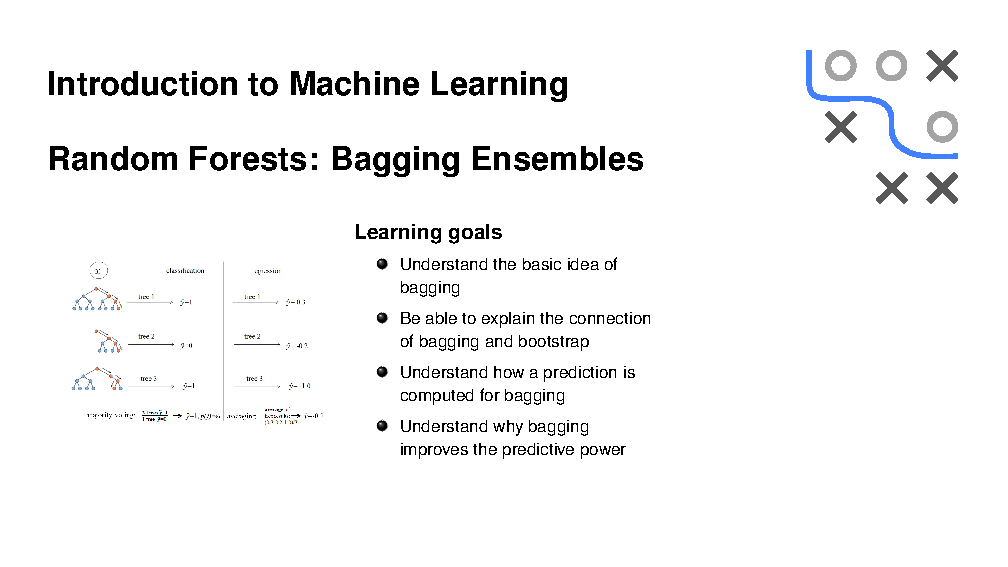
\includepdf[pages=-]{../../slides-pdf/slides-forests-bagging.pdf}

\subsection{Basics}
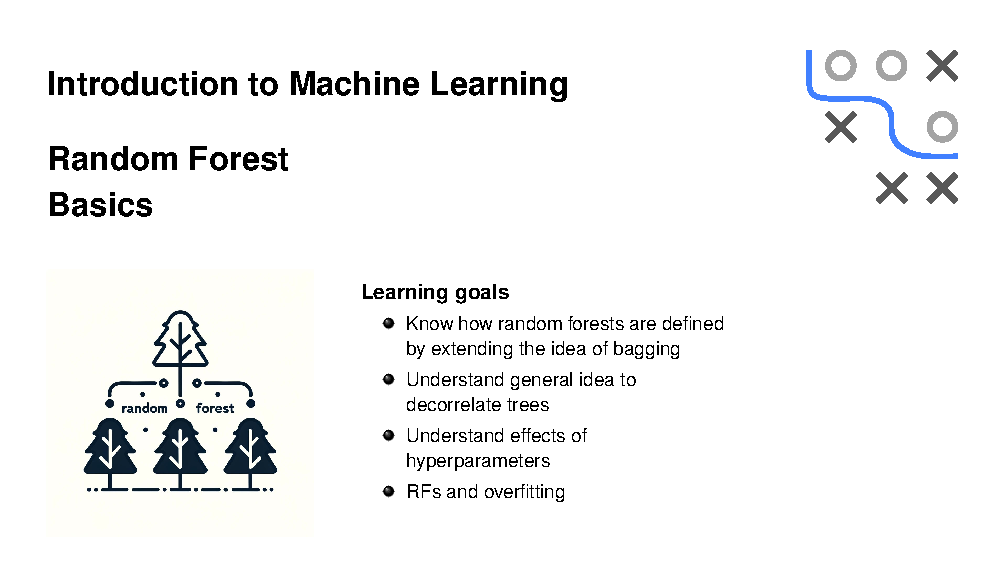
\includepdf[pages=-]{../../slides-pdf/slides-forests-basics.pdf}

\subsection{Out-of-Bag Error Estimate}
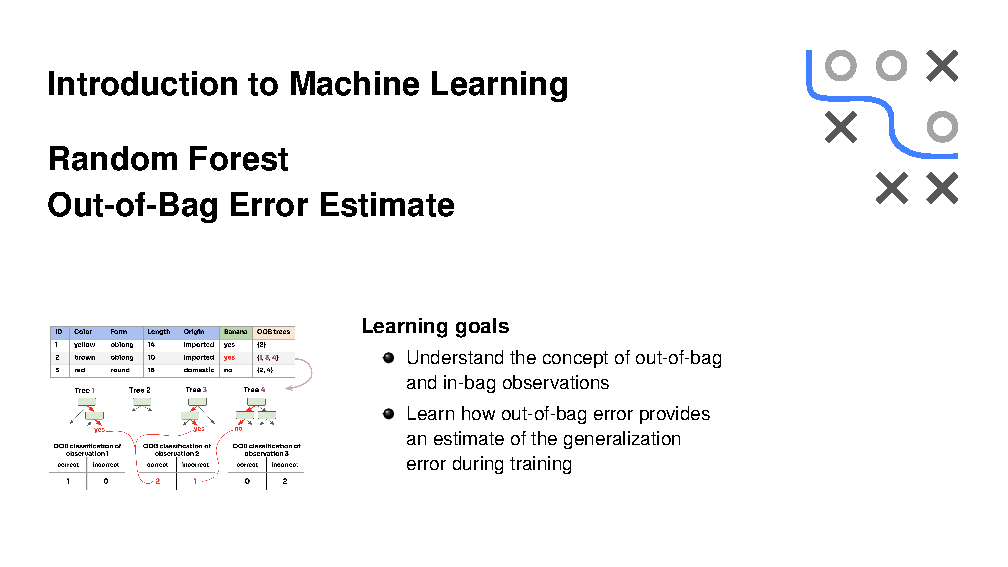
\includepdf[pages=-]{../../slides-pdf/slides-forests-oob.pdf}

\subsection{Feature Importance}
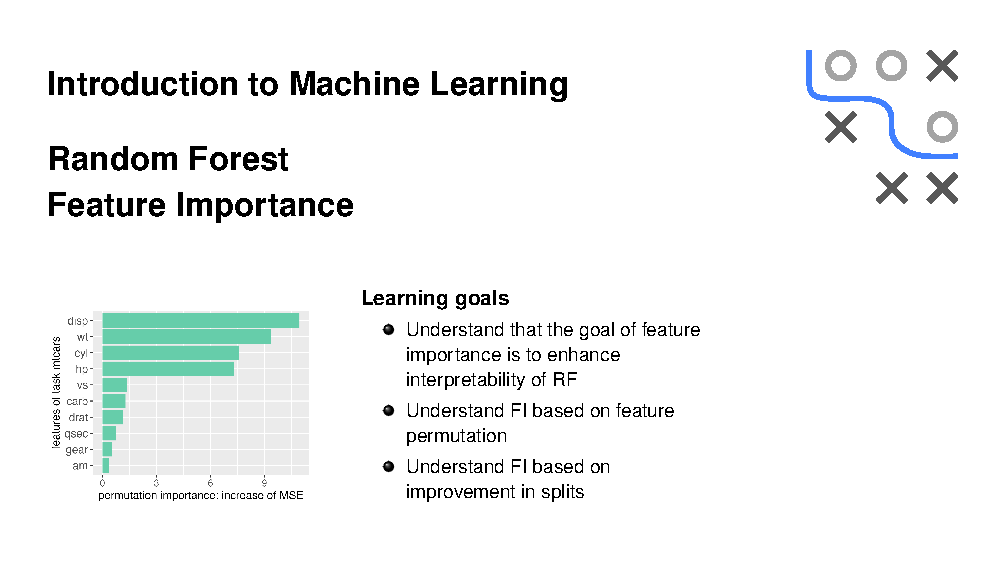
\includepdf[pages=-]{../../slides-pdf/slides-forests-featureimportance.pdf}

\subsection{Proximities}
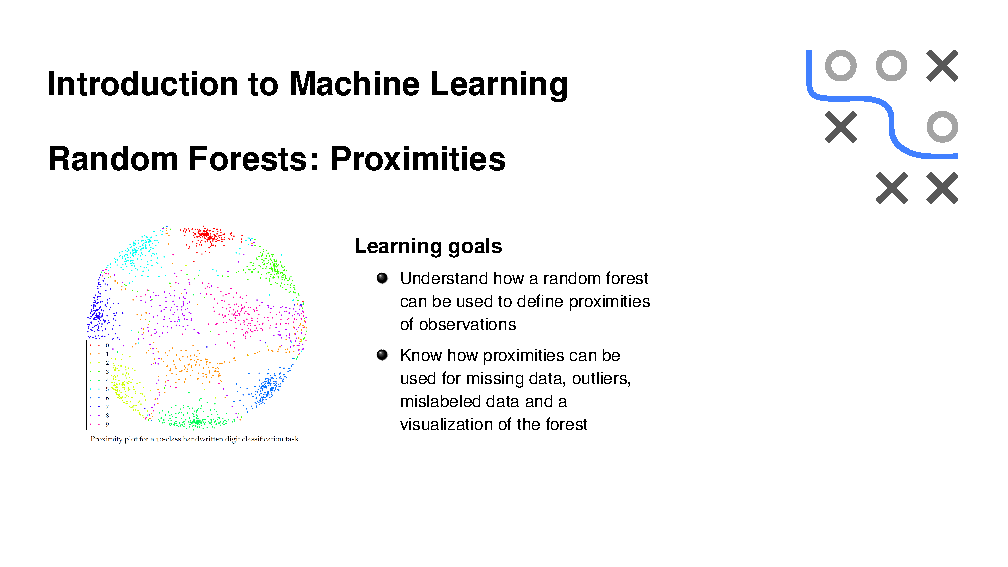
\includepdf[pages=-]{../../slides-pdf/slides-forests-proximities.pdf}

% \subsection{Bagging: Deep Dive}
% 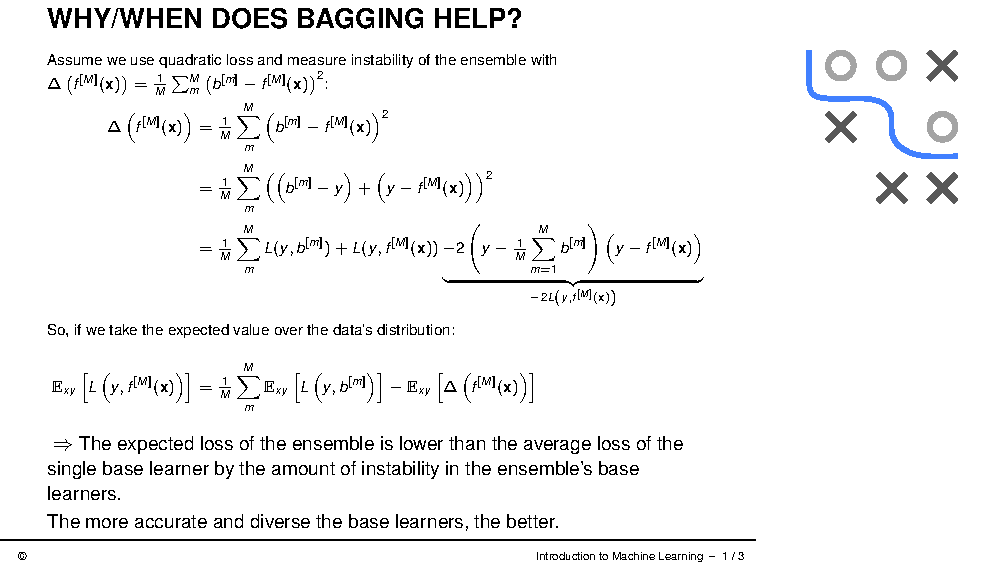
\includepdf[pages=-]{../../slides-pdf/slides-forests-bagging-deepdive.pdf}


\section{Multiclass Classification}
%Suggested order of slides:

%1 slides-forests-bagging
%2 slides-forests-basics
%3 slides-forests-oob
%4 slides-forests-featureimportance
%5 slides-forests-proximities

\subsection{Bagging Ensembles}
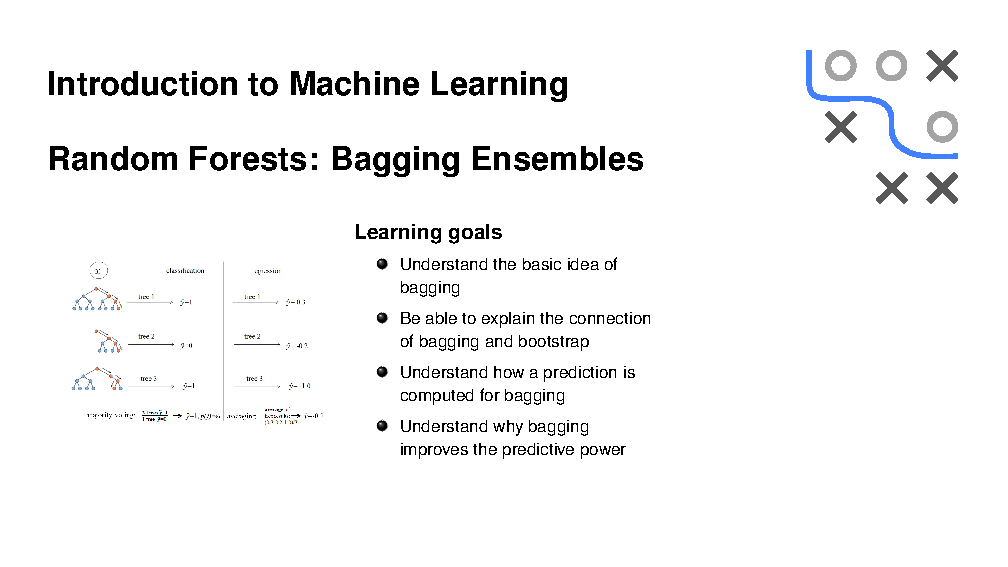
\includepdf[pages=-]{../../slides-pdf/slides-forests-bagging.pdf}

\subsection{Basics}
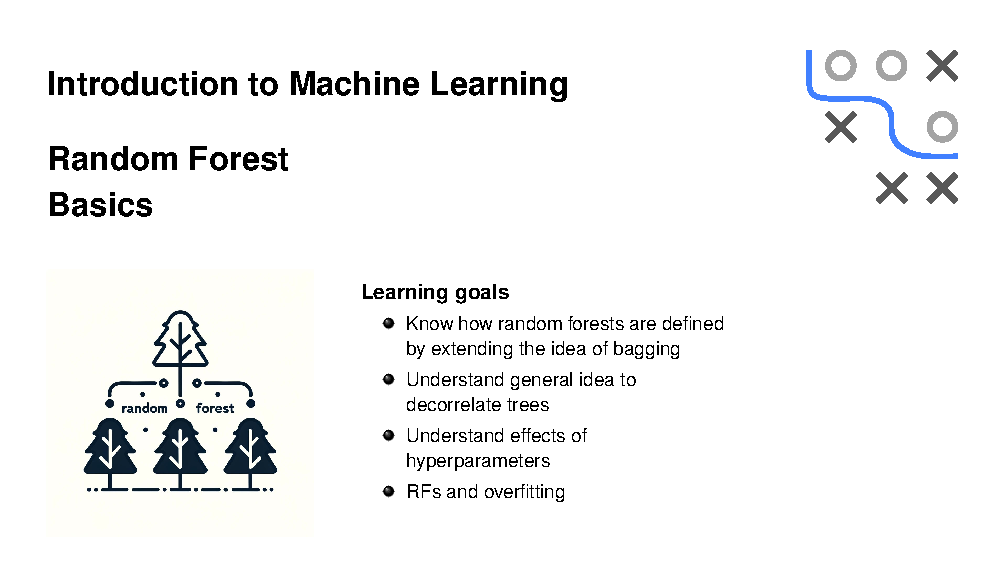
\includepdf[pages=-]{../../slides-pdf/slides-forests-basics.pdf}

\subsection{Out-of-Bag Error Estimate}
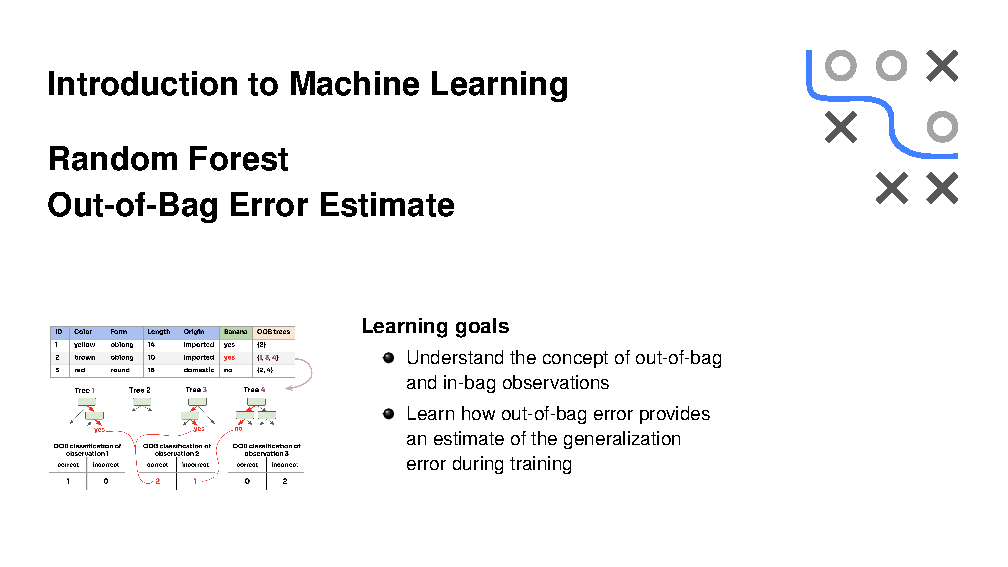
\includepdf[pages=-]{../../slides-pdf/slides-forests-oob.pdf}

\subsection{Feature Importance}
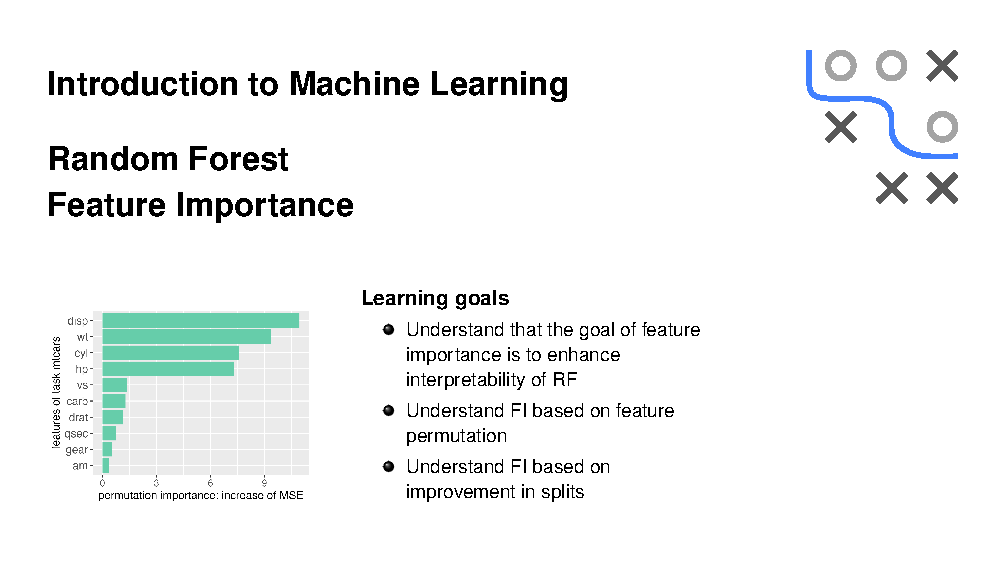
\includepdf[pages=-]{../../slides-pdf/slides-forests-featureimportance.pdf}

\subsection{Proximities}
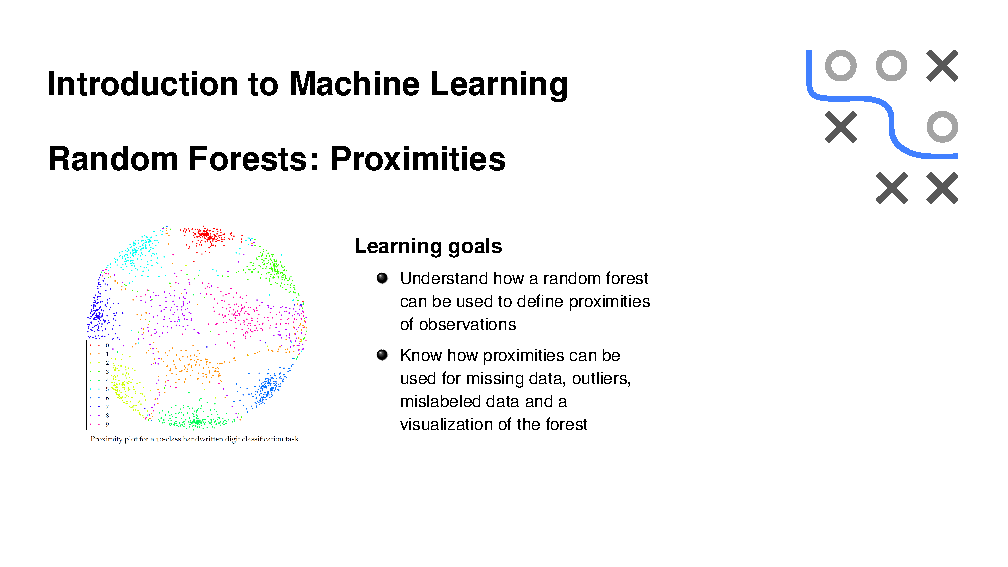
\includepdf[pages=-]{../../slides-pdf/slides-forests-proximities.pdf}

% \subsection{Bagging: Deep Dive}
% 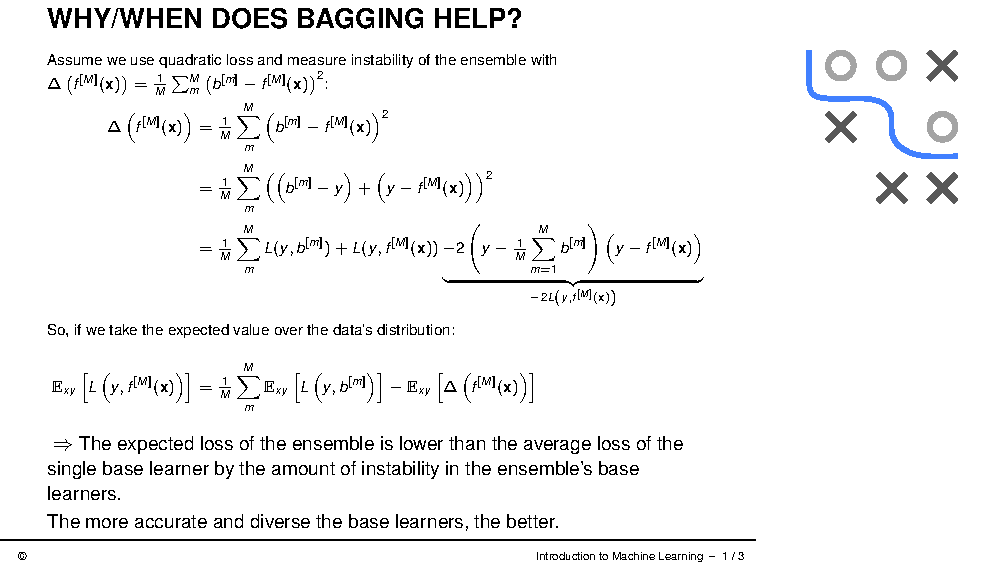
\includepdf[pages=-]{../../slides-pdf/slides-forests-bagging-deepdive.pdf}


\section{Information Theory}
%Suggested order of slides:

%1 slides-forests-bagging
%2 slides-forests-basics
%3 slides-forests-oob
%4 slides-forests-featureimportance
%5 slides-forests-proximities

\subsection{Bagging Ensembles}
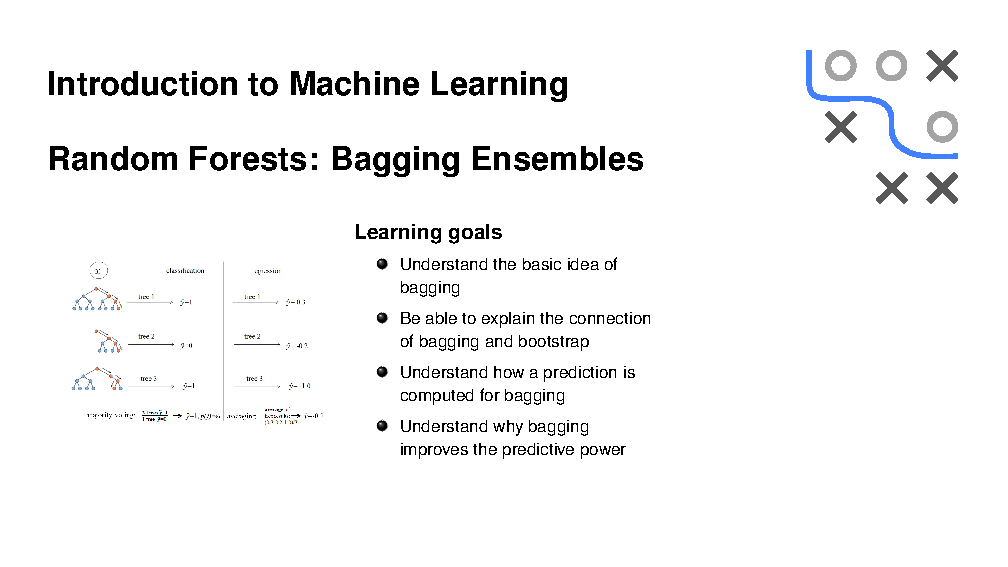
\includepdf[pages=-]{../../slides-pdf/slides-forests-bagging.pdf}

\subsection{Basics}
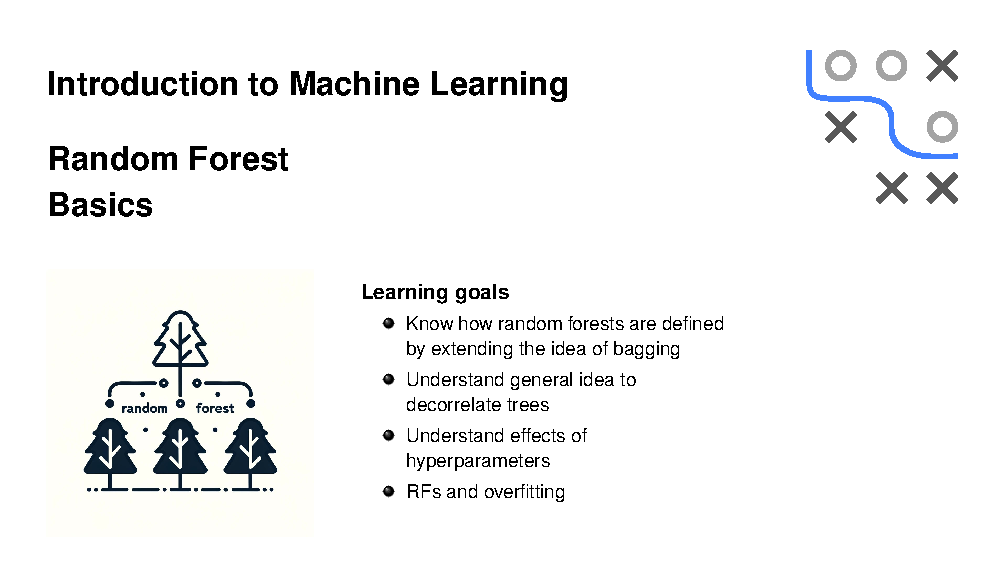
\includepdf[pages=-]{../../slides-pdf/slides-forests-basics.pdf}

\subsection{Out-of-Bag Error Estimate}
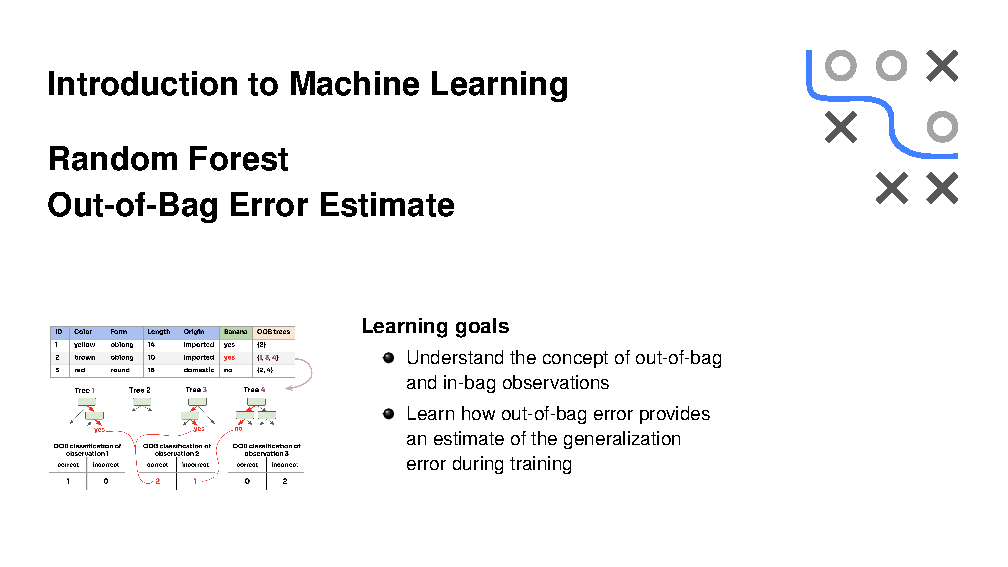
\includepdf[pages=-]{../../slides-pdf/slides-forests-oob.pdf}

\subsection{Feature Importance}
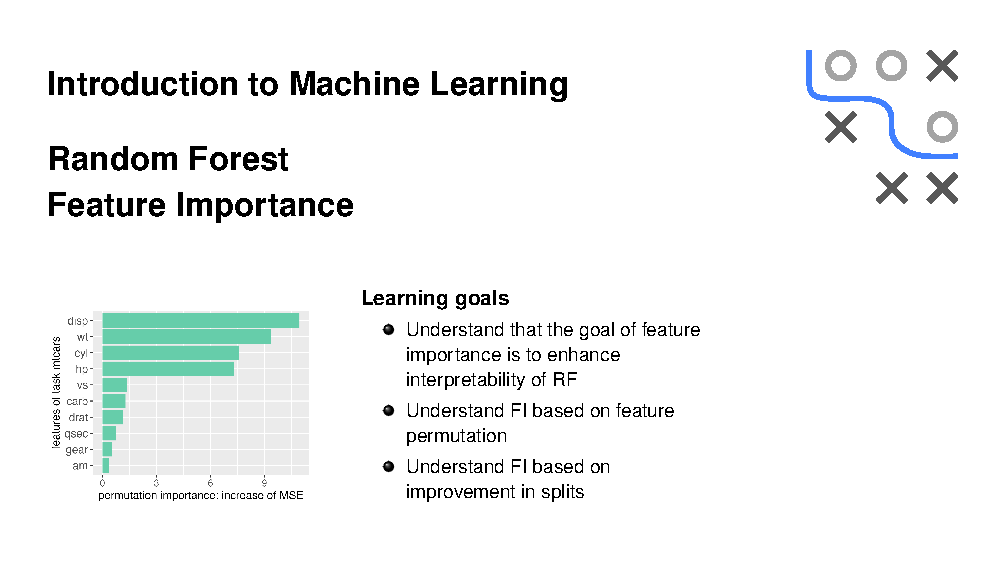
\includepdf[pages=-]{../../slides-pdf/slides-forests-featureimportance.pdf}

\subsection{Proximities}
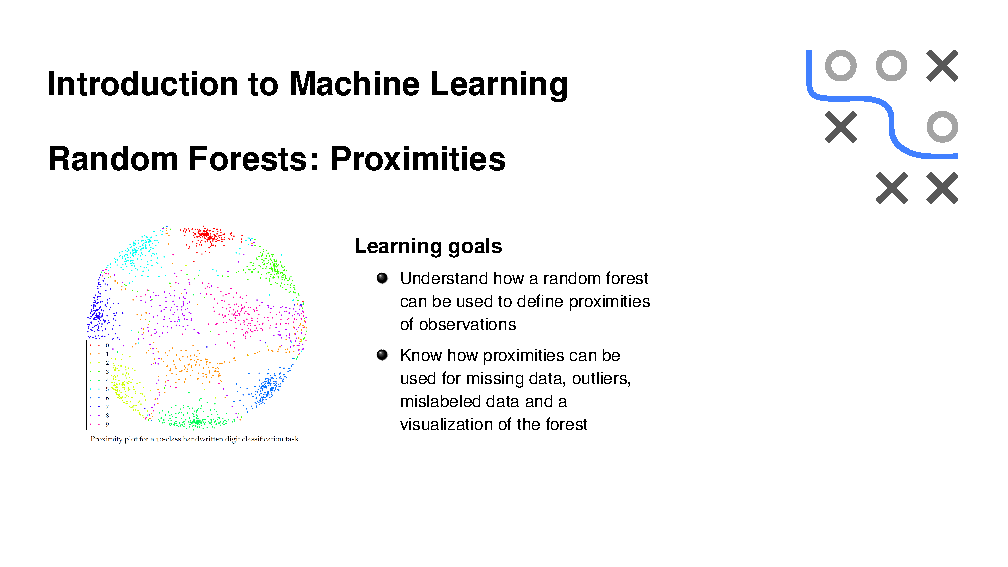
\includepdf[pages=-]{../../slides-pdf/slides-forests-proximities.pdf}

% \subsection{Bagging: Deep Dive}
% 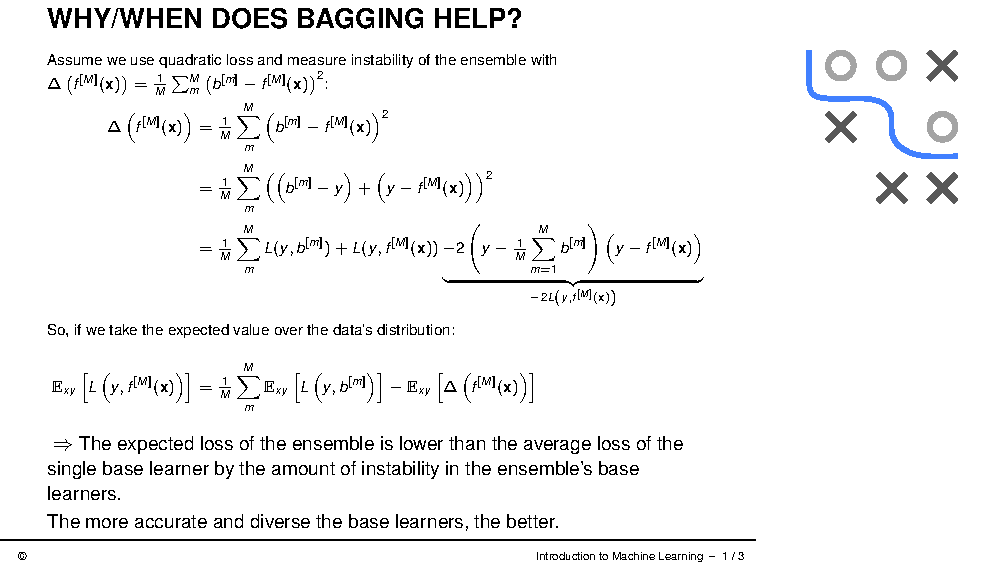
\includepdf[pages=-]{../../slides-pdf/slides-forests-bagging-deepdive.pdf}


\section{Curse of Dimensionality}
%Suggested order of slides:

%1 slides-forests-bagging
%2 slides-forests-basics
%3 slides-forests-oob
%4 slides-forests-featureimportance
%5 slides-forests-proximities

\subsection{Bagging Ensembles}
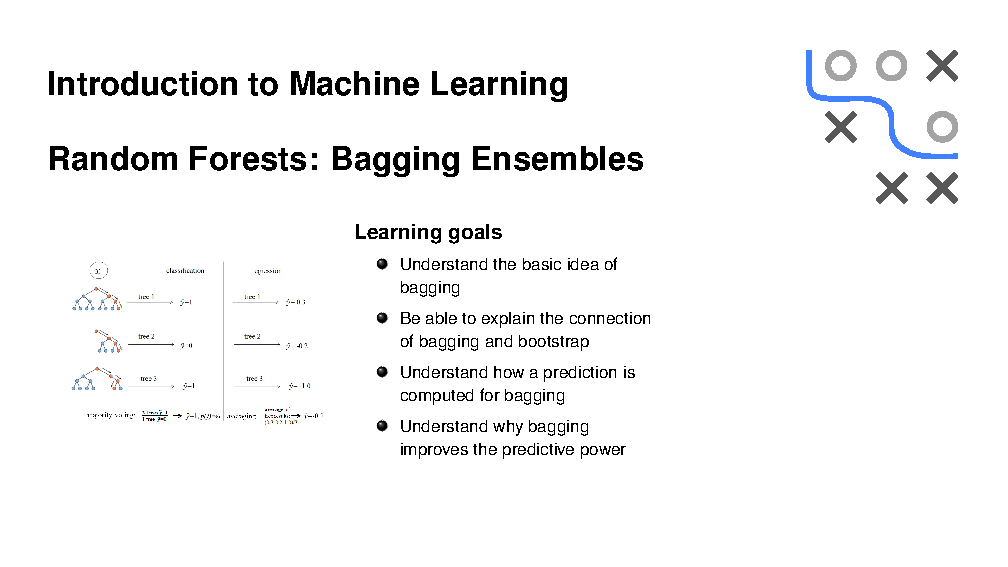
\includepdf[pages=-]{../../slides-pdf/slides-forests-bagging.pdf}

\subsection{Basics}
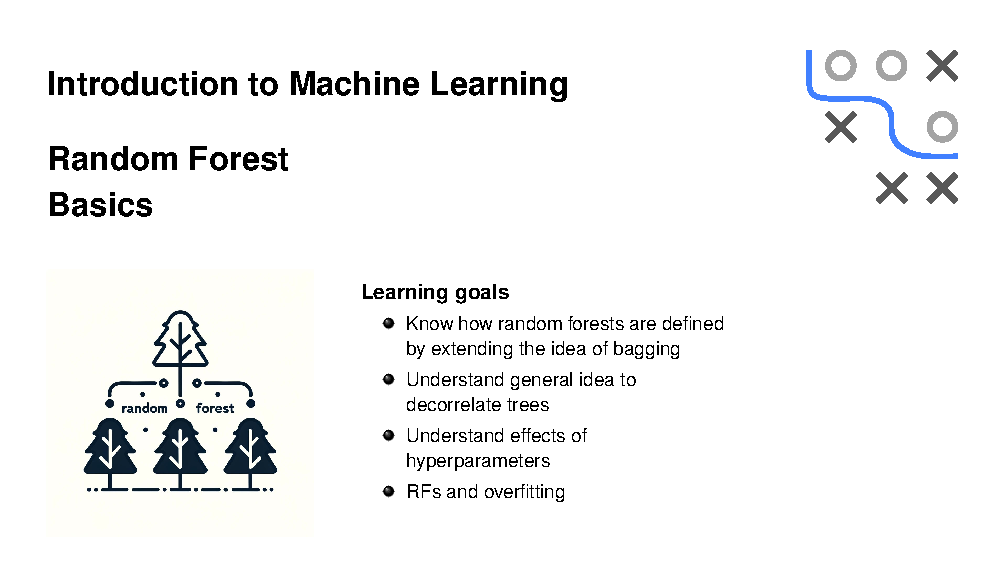
\includepdf[pages=-]{../../slides-pdf/slides-forests-basics.pdf}

\subsection{Out-of-Bag Error Estimate}
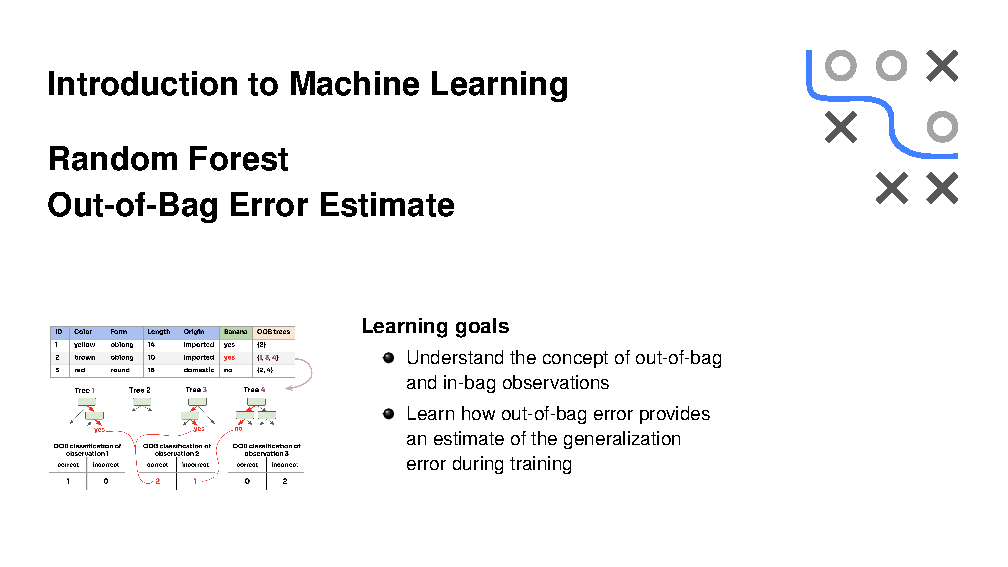
\includepdf[pages=-]{../../slides-pdf/slides-forests-oob.pdf}

\subsection{Feature Importance}
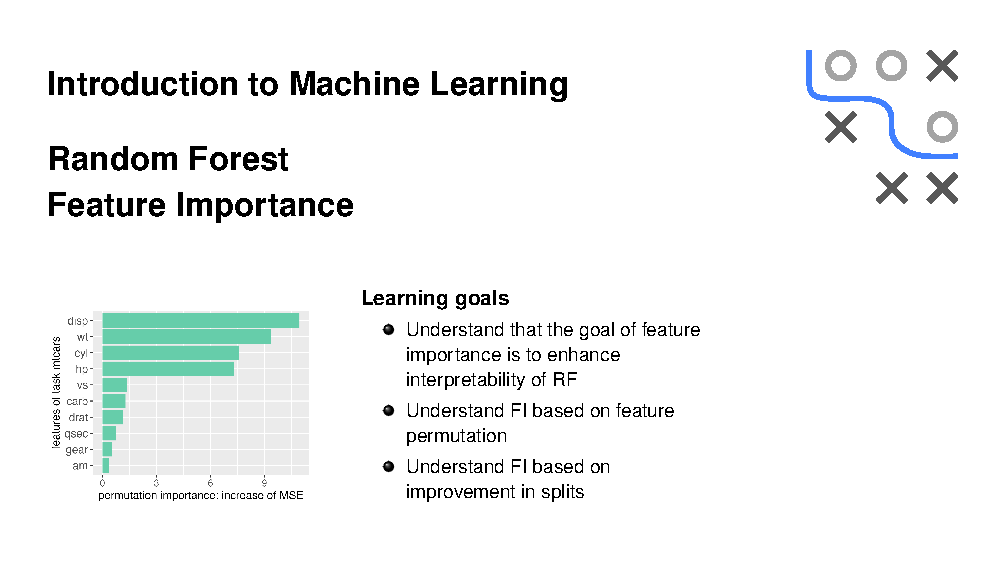
\includepdf[pages=-]{../../slides-pdf/slides-forests-featureimportance.pdf}

\subsection{Proximities}
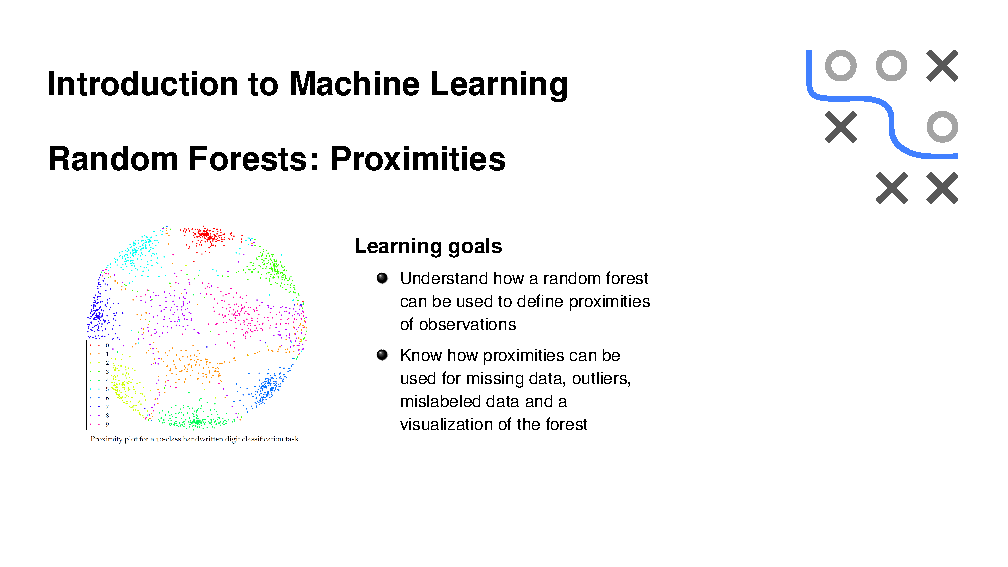
\includepdf[pages=-]{../../slides-pdf/slides-forests-proximities.pdf}

% \subsection{Bagging: Deep Dive}
% 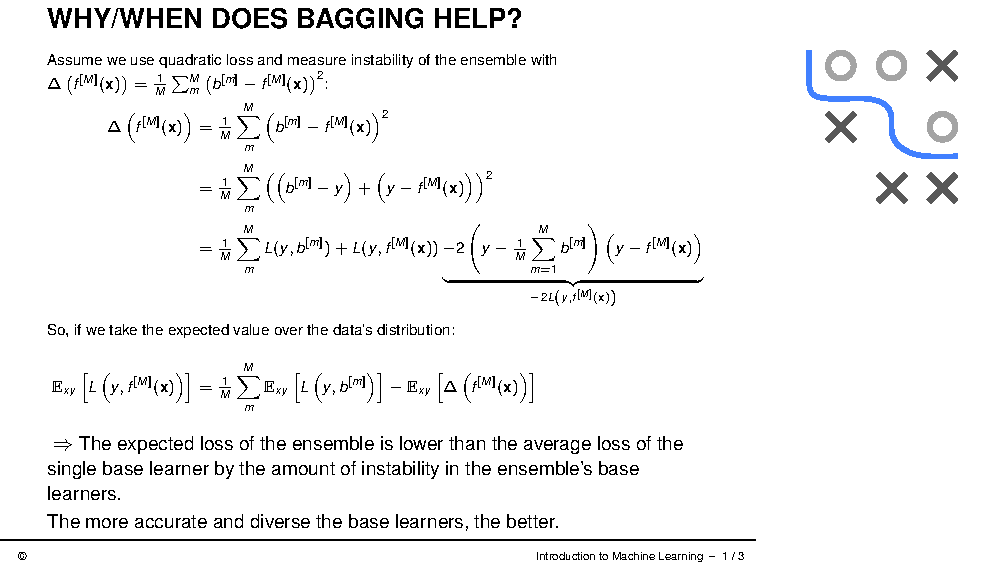
\includepdf[pages=-]{../../slides-pdf/slides-forests-bagging-deepdive.pdf}


\section{Hypothesis Space}
%Suggested order of slides:

%1 slides-forests-bagging
%2 slides-forests-basics
%3 slides-forests-oob
%4 slides-forests-featureimportance
%5 slides-forests-proximities

\subsection{Bagging Ensembles}
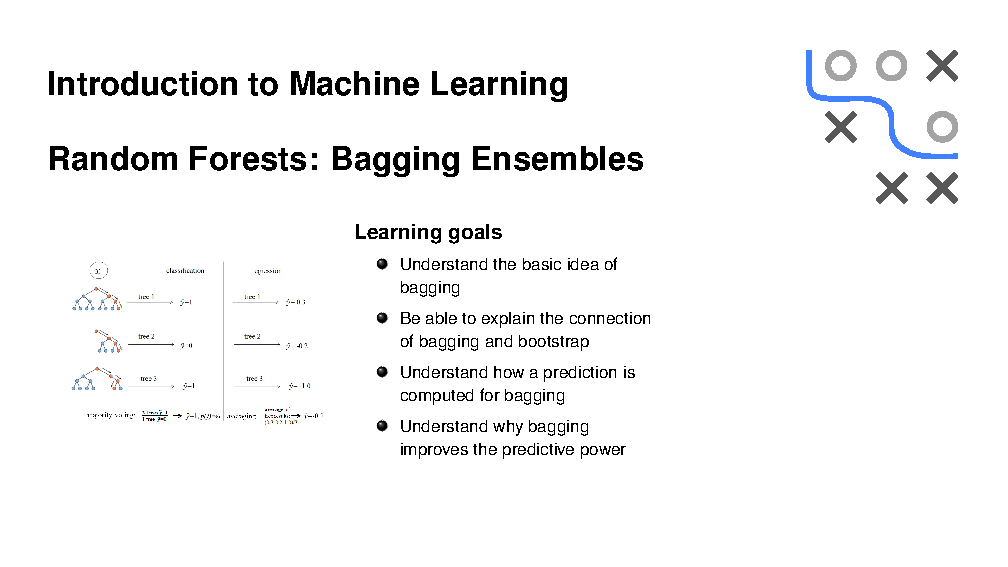
\includepdf[pages=-]{../../slides-pdf/slides-forests-bagging.pdf}

\subsection{Basics}
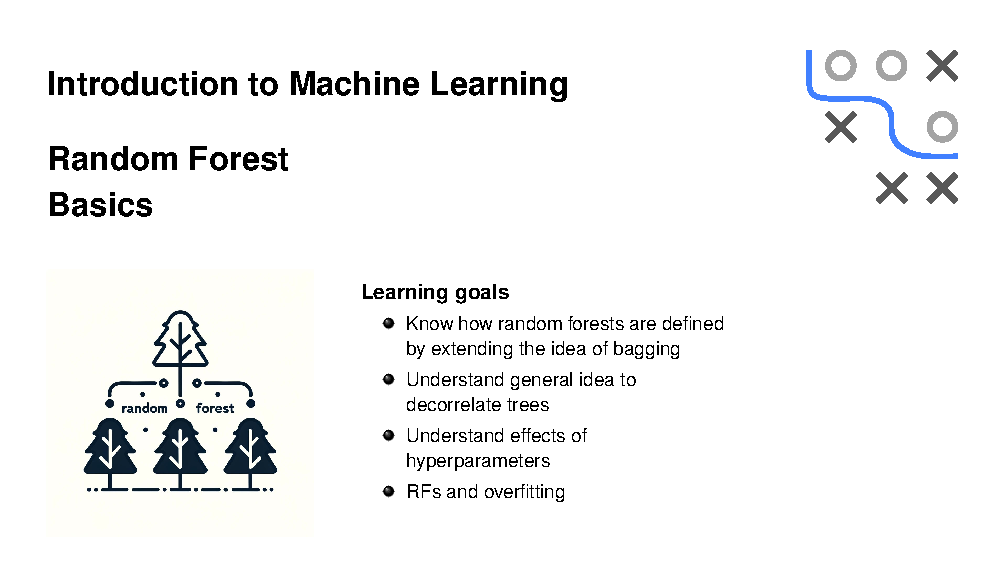
\includepdf[pages=-]{../../slides-pdf/slides-forests-basics.pdf}

\subsection{Out-of-Bag Error Estimate}
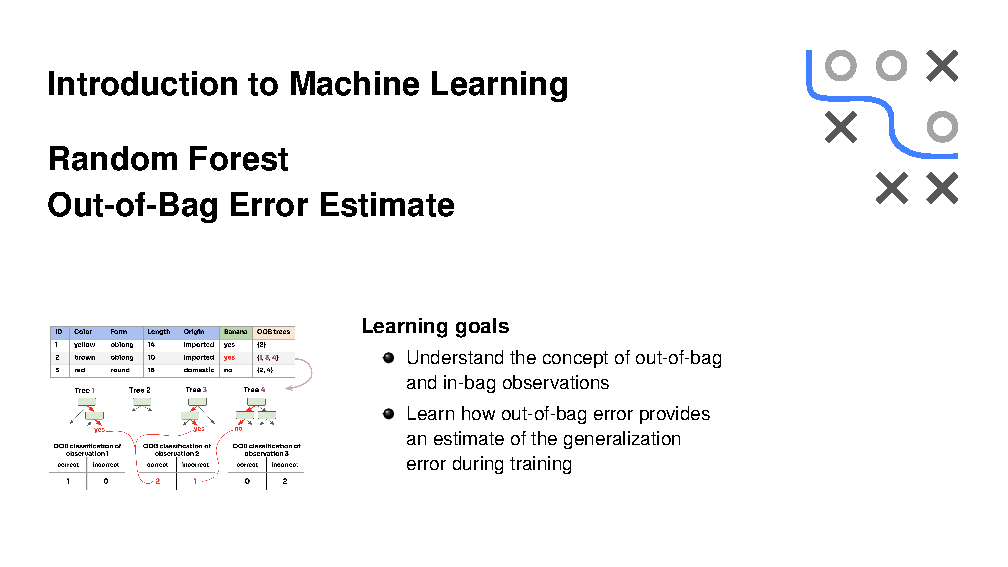
\includepdf[pages=-]{../../slides-pdf/slides-forests-oob.pdf}

\subsection{Feature Importance}
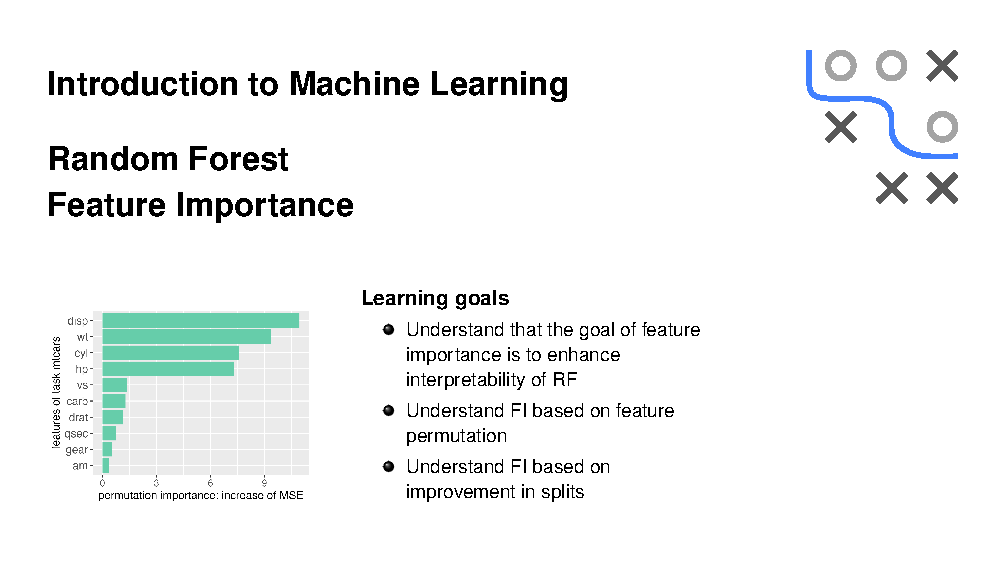
\includepdf[pages=-]{../../slides-pdf/slides-forests-featureimportance.pdf}

\subsection{Proximities}
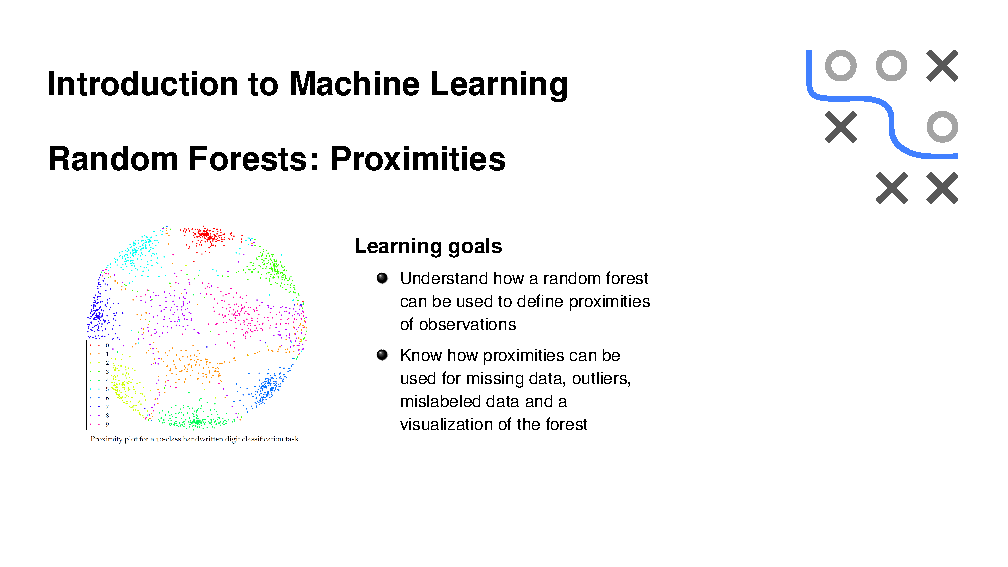
\includepdf[pages=-]{../../slides-pdf/slides-forests-proximities.pdf}

% \subsection{Bagging: Deep Dive}
% 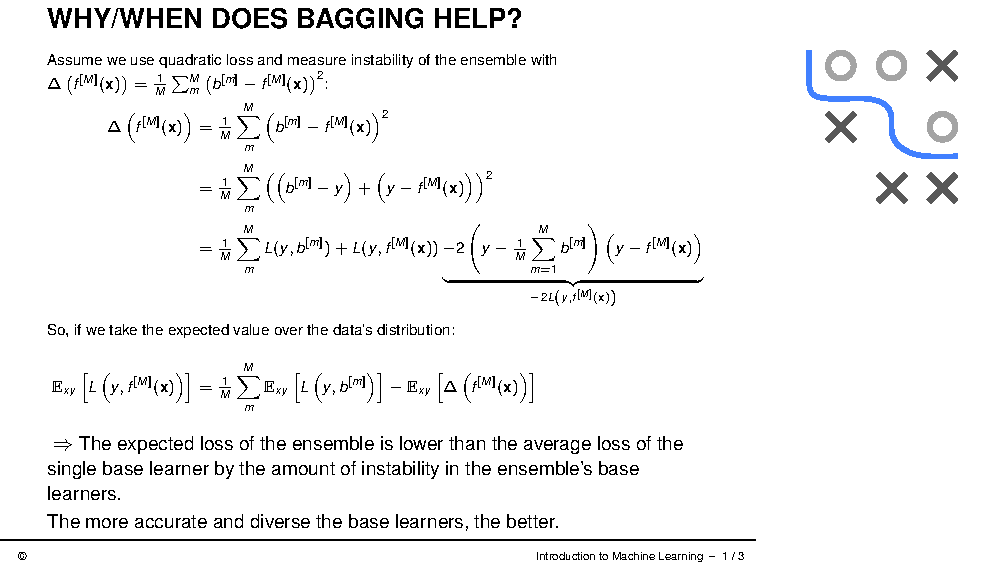
\includepdf[pages=-]{../../slides-pdf/slides-forests-bagging-deepdive.pdf}


\section{Regularization}
%Suggested order of slides:

%1 slides-forests-bagging
%2 slides-forests-basics
%3 slides-forests-oob
%4 slides-forests-featureimportance
%5 slides-forests-proximities

\subsection{Bagging Ensembles}
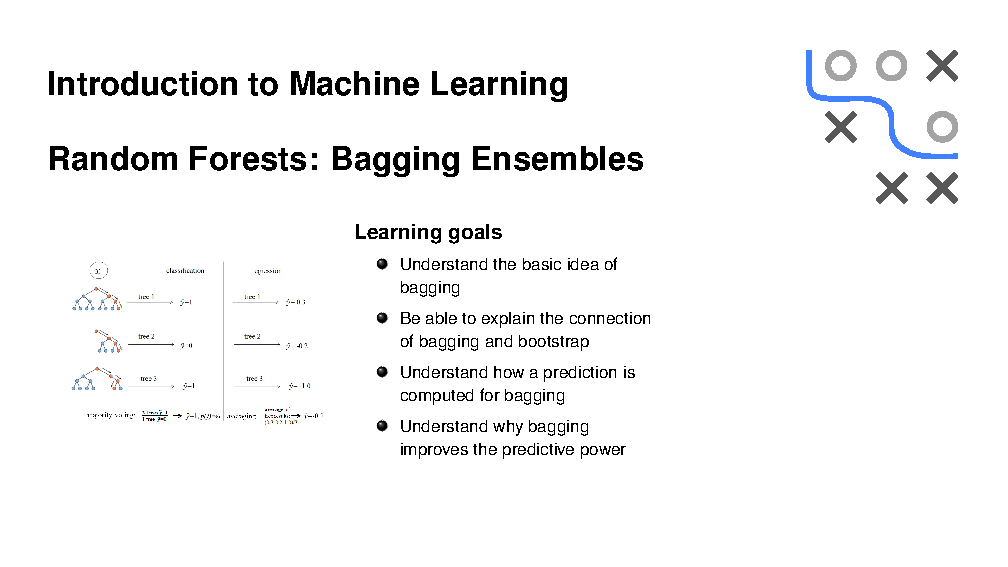
\includepdf[pages=-]{../../slides-pdf/slides-forests-bagging.pdf}

\subsection{Basics}
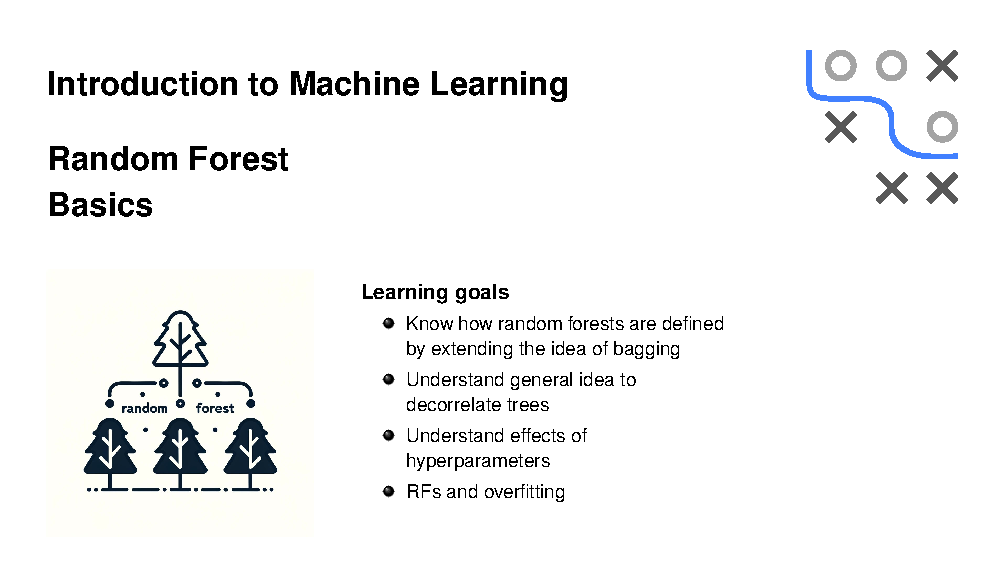
\includepdf[pages=-]{../../slides-pdf/slides-forests-basics.pdf}

\subsection{Out-of-Bag Error Estimate}
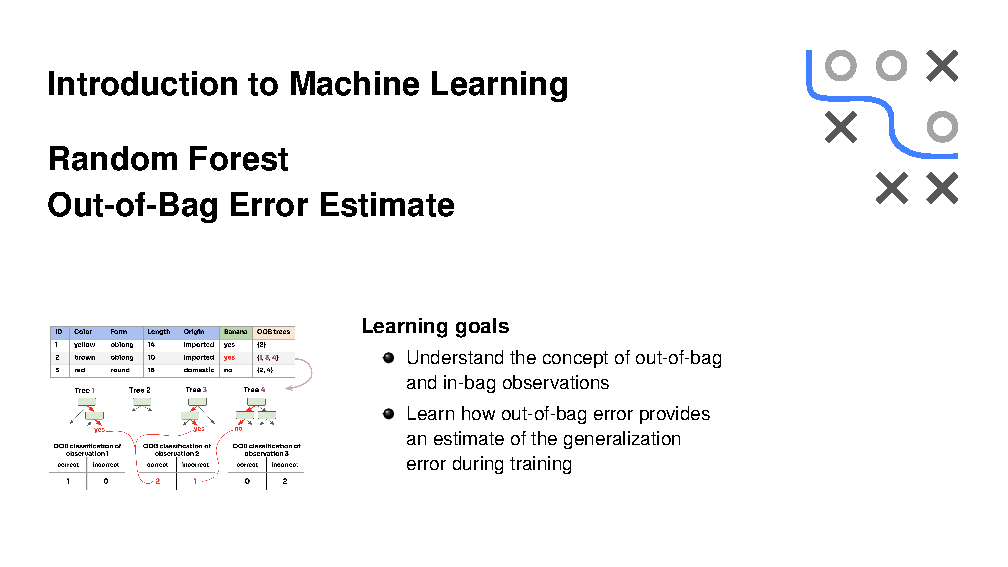
\includepdf[pages=-]{../../slides-pdf/slides-forests-oob.pdf}

\subsection{Feature Importance}
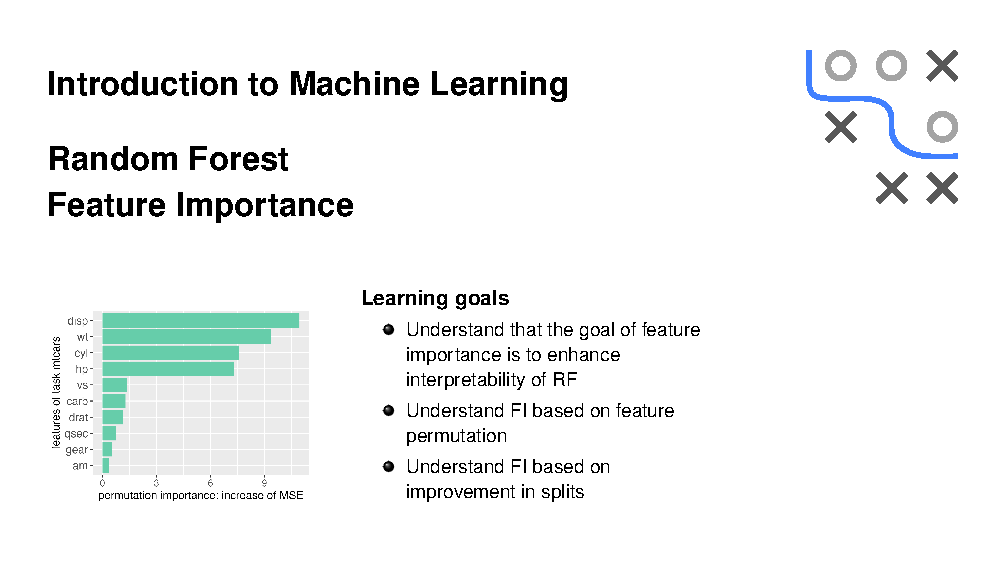
\includepdf[pages=-]{../../slides-pdf/slides-forests-featureimportance.pdf}

\subsection{Proximities}
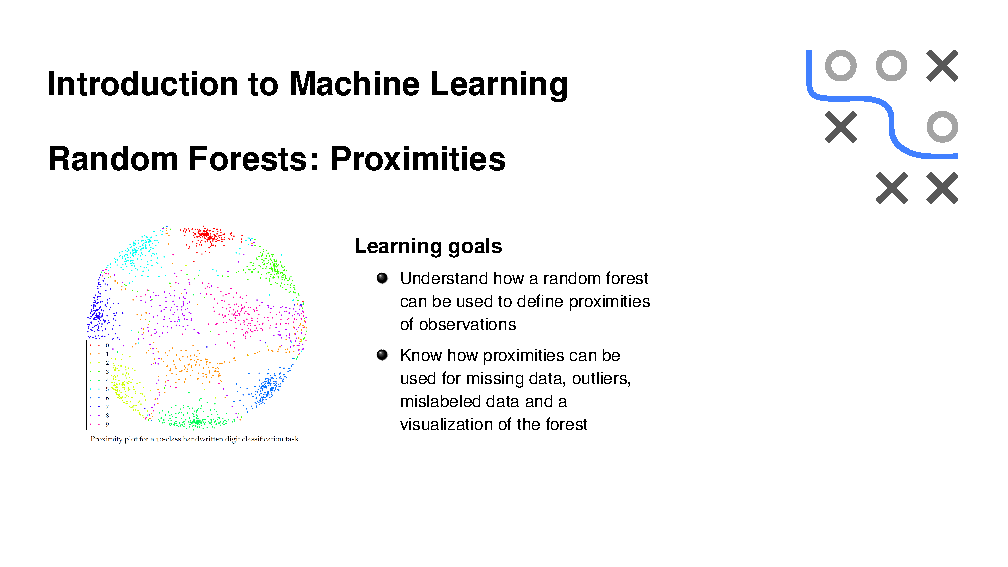
\includepdf[pages=-]{../../slides-pdf/slides-forests-proximities.pdf}

% \subsection{Bagging: Deep Dive}
% 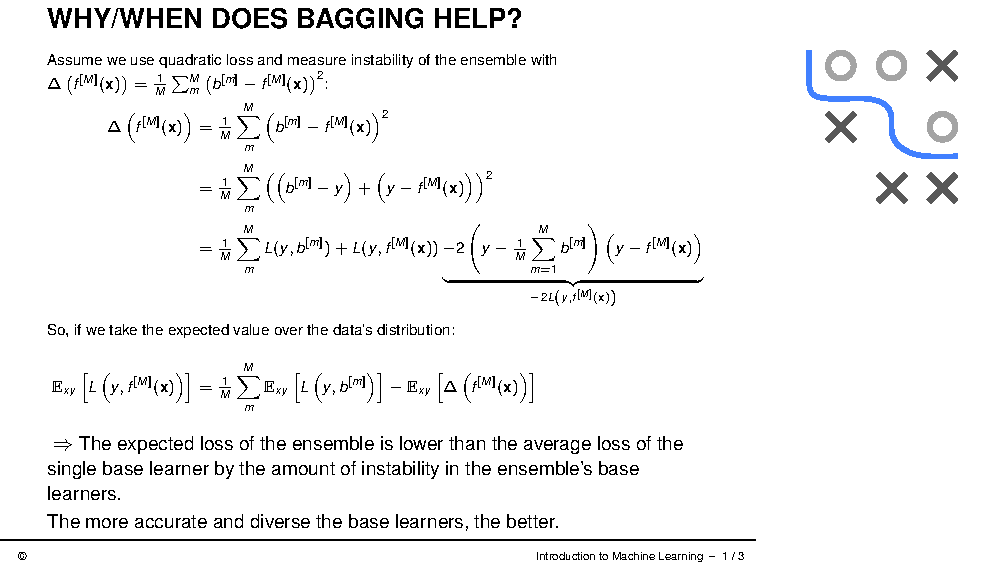
\includepdf[pages=-]{../../slides-pdf/slides-forests-bagging-deepdive.pdf}


\section{Linear Support Vector Machine}
%Suggested order of slides:

%1 slides-forests-bagging
%2 slides-forests-basics
%3 slides-forests-oob
%4 slides-forests-featureimportance
%5 slides-forests-proximities

\subsection{Bagging Ensembles}
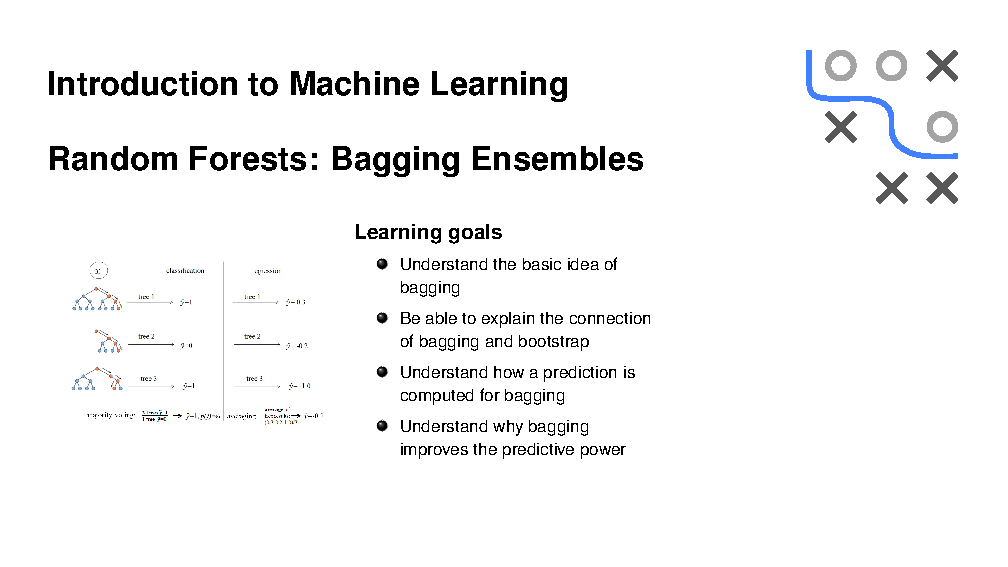
\includepdf[pages=-]{../../slides-pdf/slides-forests-bagging.pdf}

\subsection{Basics}
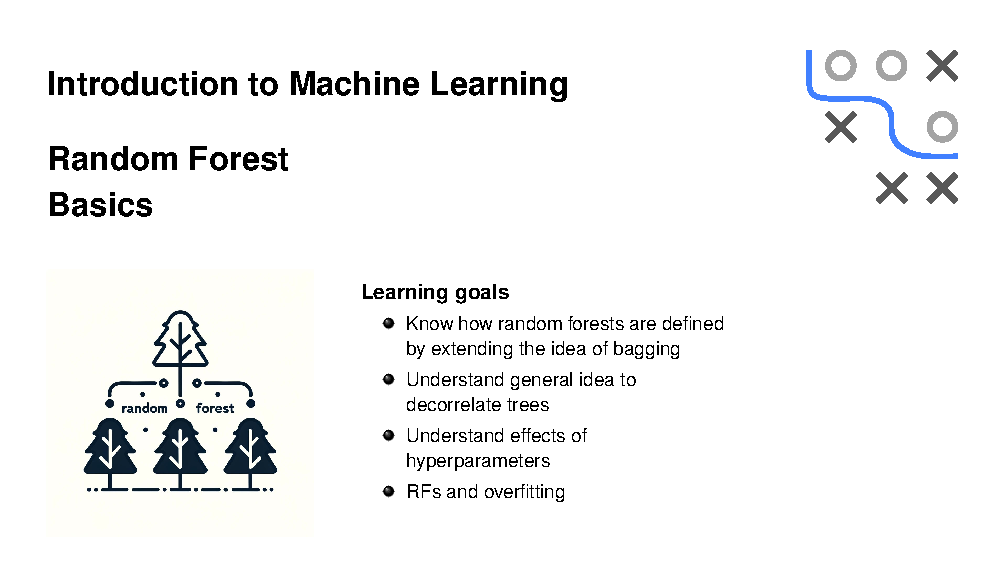
\includepdf[pages=-]{../../slides-pdf/slides-forests-basics.pdf}

\subsection{Out-of-Bag Error Estimate}
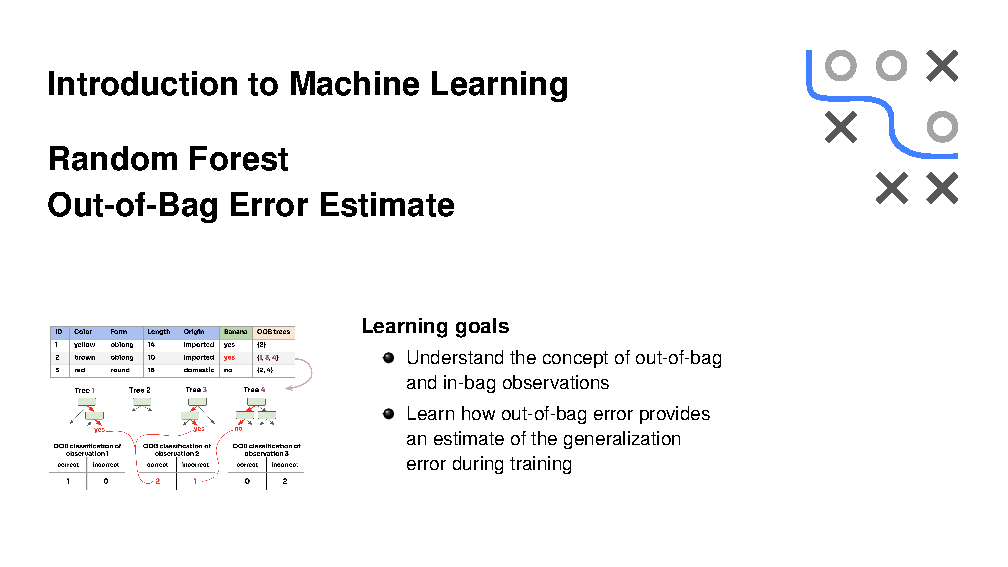
\includepdf[pages=-]{../../slides-pdf/slides-forests-oob.pdf}

\subsection{Feature Importance}
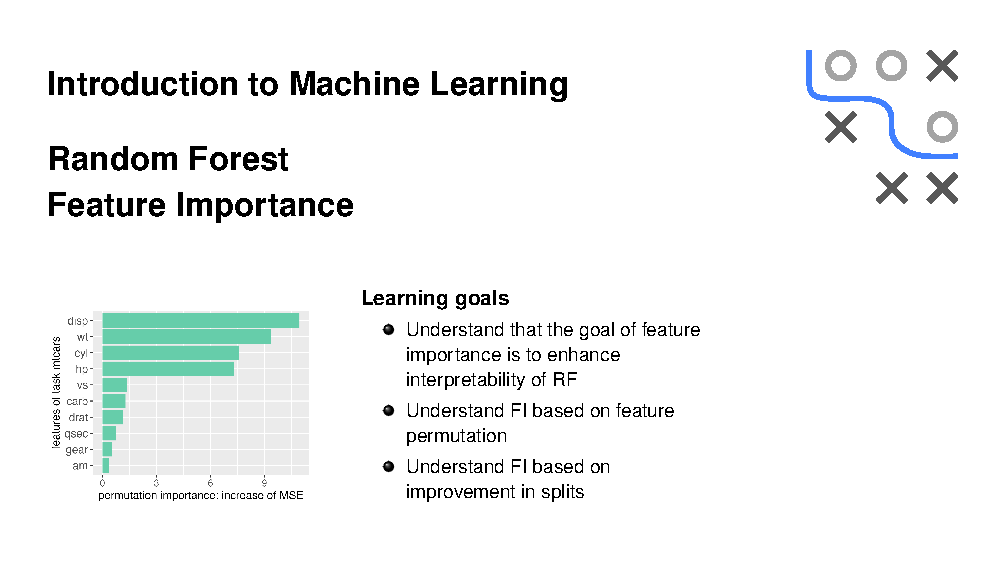
\includepdf[pages=-]{../../slides-pdf/slides-forests-featureimportance.pdf}

\subsection{Proximities}
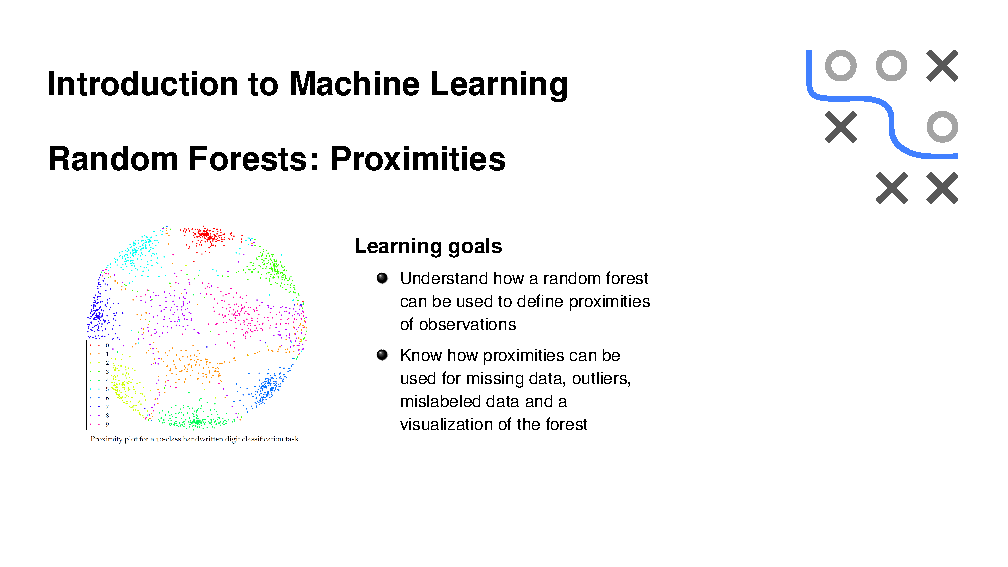
\includepdf[pages=-]{../../slides-pdf/slides-forests-proximities.pdf}

% \subsection{Bagging: Deep Dive}
% 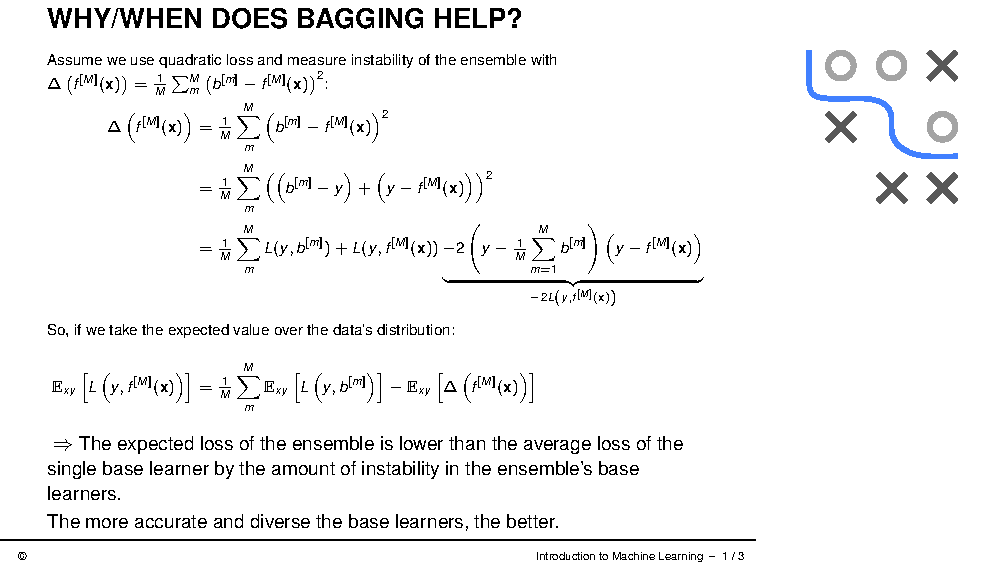
\includepdf[pages=-]{../../slides-pdf/slides-forests-bagging-deepdive.pdf}


\section{Nonlinear Support Vector Machine}
%Suggested order of slides:

%1 slides-forests-bagging
%2 slides-forests-basics
%3 slides-forests-oob
%4 slides-forests-featureimportance
%5 slides-forests-proximities

\subsection{Bagging Ensembles}
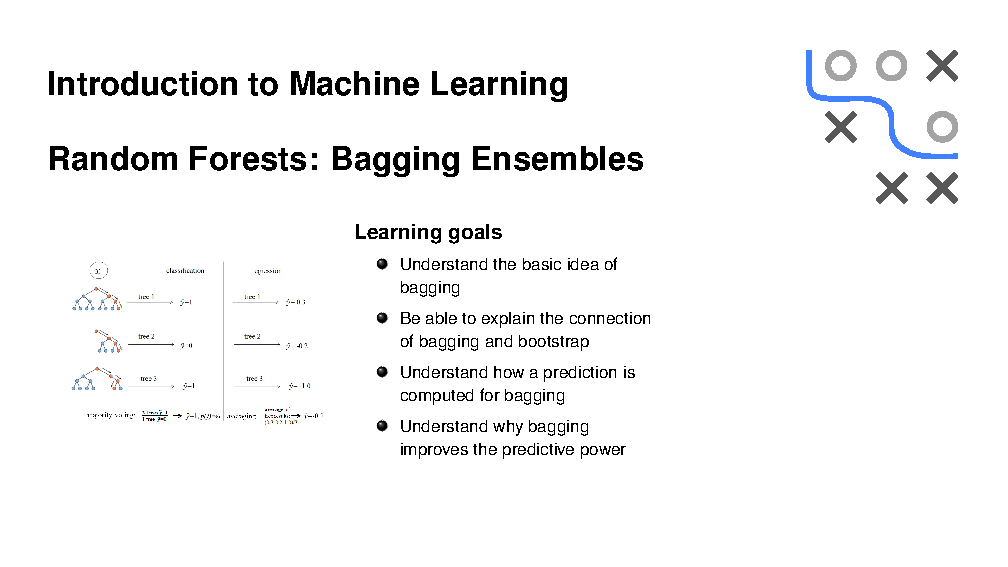
\includepdf[pages=-]{../../slides-pdf/slides-forests-bagging.pdf}

\subsection{Basics}
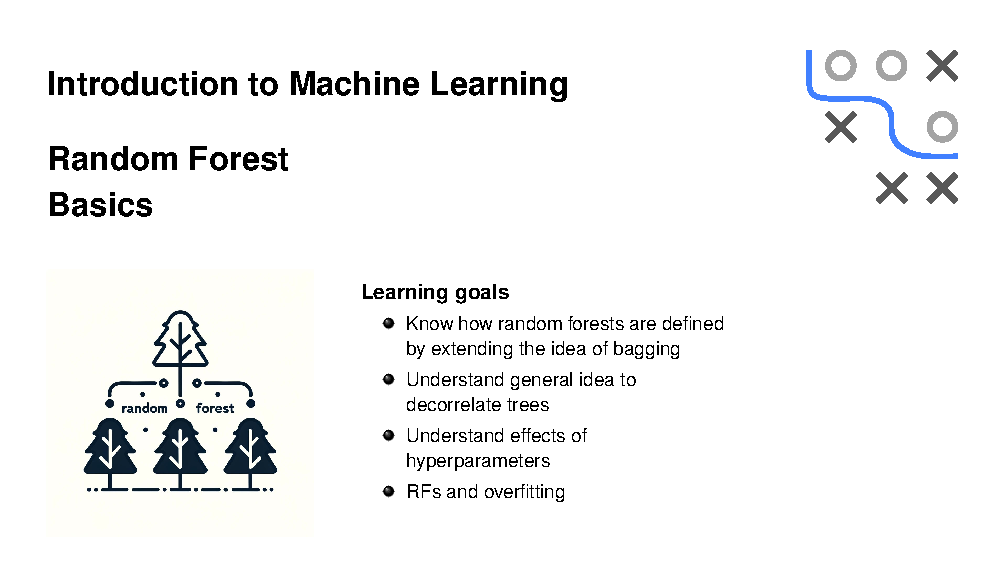
\includepdf[pages=-]{../../slides-pdf/slides-forests-basics.pdf}

\subsection{Out-of-Bag Error Estimate}
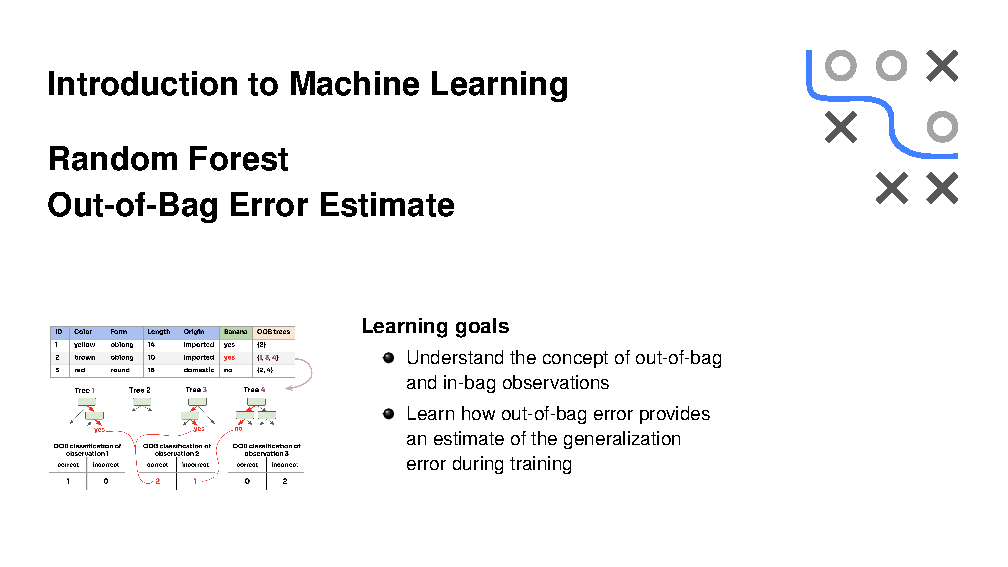
\includepdf[pages=-]{../../slides-pdf/slides-forests-oob.pdf}

\subsection{Feature Importance}
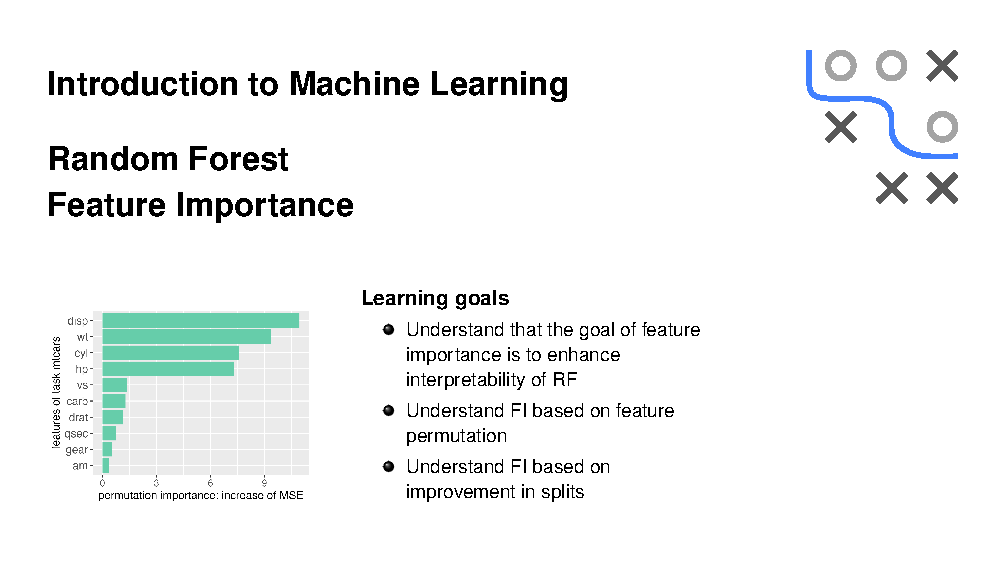
\includepdf[pages=-]{../../slides-pdf/slides-forests-featureimportance.pdf}

\subsection{Proximities}
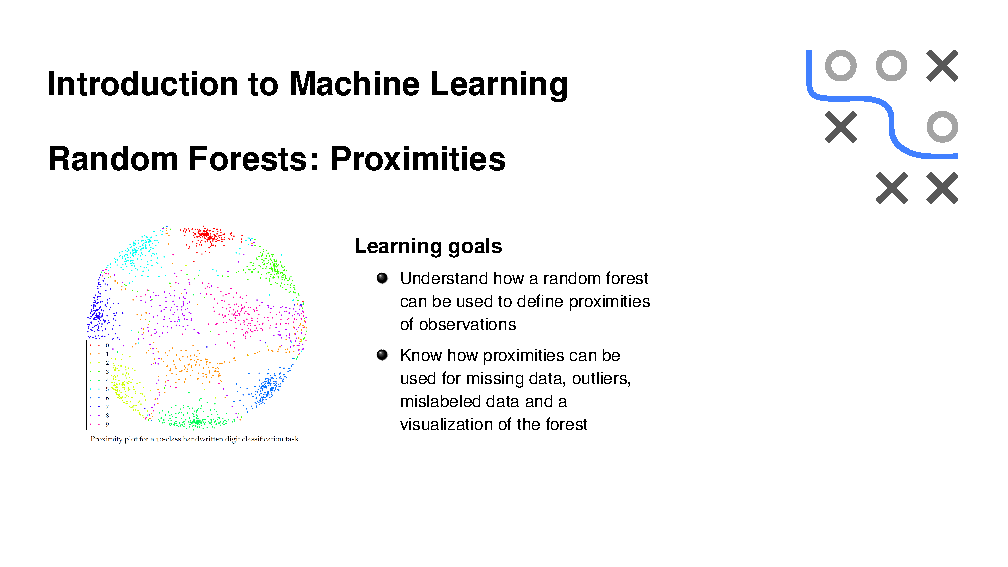
\includepdf[pages=-]{../../slides-pdf/slides-forests-proximities.pdf}

% \subsection{Bagging: Deep Dive}
% 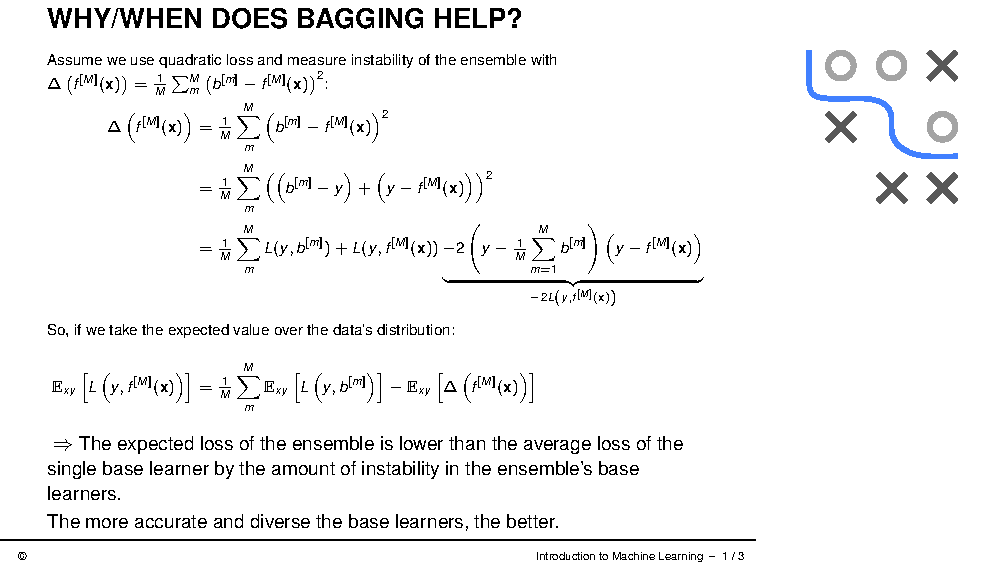
\includepdf[pages=-]{../../slides-pdf/slides-forests-bagging-deepdive.pdf}


\section{Gaussian Processes}
%Suggested order of slides:

%1 slides-forests-bagging
%2 slides-forests-basics
%3 slides-forests-oob
%4 slides-forests-featureimportance
%5 slides-forests-proximities

\subsection{Bagging Ensembles}
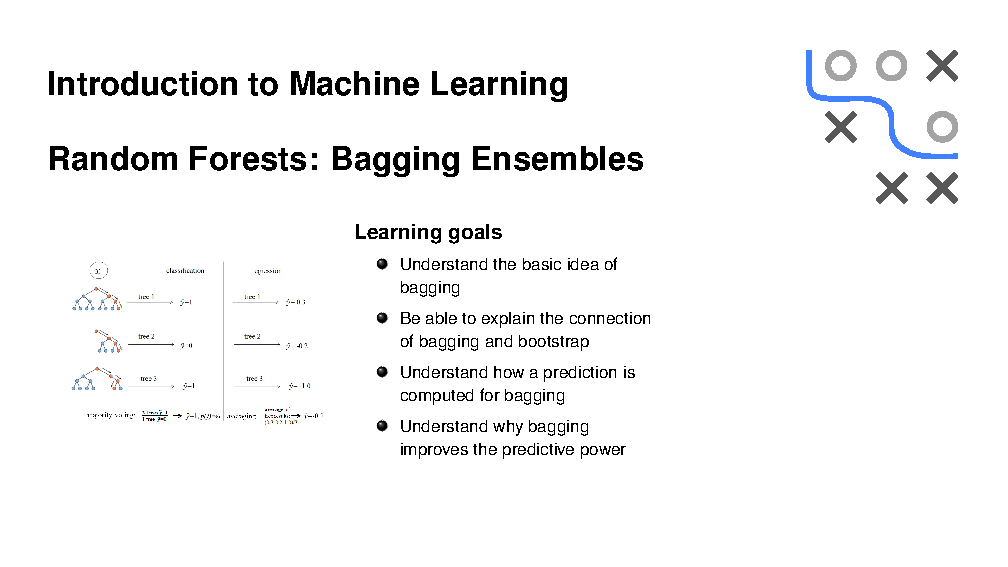
\includepdf[pages=-]{../../slides-pdf/slides-forests-bagging.pdf}

\subsection{Basics}
\includepdf[pages=-]{../../slides-pdf/slides-forests-basics.pdf}

\subsection{Out-of-Bag Error Estimate}
\includepdf[pages=-]{../../slides-pdf/slides-forests-oob.pdf}

\subsection{Feature Importance}
\includepdf[pages=-]{../../slides-pdf/slides-forests-featureimportance.pdf}

\subsection{Proximities}
\includepdf[pages=-]{../../slides-pdf/slides-forests-proximities.pdf}

% \subsection{Bagging: Deep Dive}
% \includepdf[pages=-]{../../slides-pdf/slides-forests-bagging-deepdive.pdf}


\section{Boosting}
%Suggested order of slides:

%1 slides-forests-bagging
%2 slides-forests-basics
%3 slides-forests-oob
%4 slides-forests-featureimportance
%5 slides-forests-proximities

\subsection{Bagging Ensembles}
\includepdf[pages=-]{../../slides-pdf/slides-forests-bagging.pdf}

\subsection{Basics}
\includepdf[pages=-]{../../slides-pdf/slides-forests-basics.pdf}

\subsection{Out-of-Bag Error Estimate}
\includepdf[pages=-]{../../slides-pdf/slides-forests-oob.pdf}

\subsection{Feature Importance}
\includepdf[pages=-]{../../slides-pdf/slides-forests-featureimportance.pdf}

\subsection{Proximities}
\includepdf[pages=-]{../../slides-pdf/slides-forests-proximities.pdf}

% \subsection{Bagging: Deep Dive}
% \includepdf[pages=-]{../../slides-pdf/slides-forests-bagging-deepdive.pdf}


\end{document}
